\chapter{Validación y resultados}
\label{chap:validacion-resultados}

Este capítulo recoge los resultados de la validación del sistema a lo largo de los sprints de cierre. Se documenta la estrategia de validación multicapa, las pruebas funcionales automatizadas, la validación de infraestructura cloud, los resultados obtenidos en cada sprint y el análisis de limitaciones del trabajo. La trazabilidad completa entre requisitos, implementación y evidencias se recoge en el Anexo~\ref{chap:anexo-trazabilidad}.

\section{Estrategia de validación}
\label{sec:estrategia-validacion}

La validación se ha organizado en tres niveles: pruebas de backend, validación de infraestructura y pruebas de operación sobre el entorno desplegado. Esta estrategia evita depender de una sola evidencia y permite demostrar tanto comportamiento funcional como capacidad real de despliegue.

En local se ejecutan pruebas automatizadas y flujos Postman/Newman contra una API viva. En infraestructura se usan \texttt{terraform fmt}, \texttt{terraform validate}, \texttt{terraform plan}, \texttt{terraform apply} y \texttt{terraform destroy}. En AWS se comprueba el estado de ECS, la migración puntual, la salud del endpoint, el bootstrap de administrador, el login, la existencia de recursos de observabilidad, el rollback de despliegue y el restore temporal de RDS.

\section{Pruebas funcionales}
\label{sec:pruebas-funcionales}

La suite principal de pruebas automatizadas contiene 87 pruebas superadas durante la fase de cierre. Estas pruebas cubren endpoints de salud, transportes, vehículos, conductores, autenticación, usuarios, reglas de estado y el contrato de correlación de peticiones. La validación automatizada se complementa con un flujo de smoke local basado en Postman/Newman, que arranca Docker Compose, prepara datos deterministas, ejecuta peticiones y limpia los datos generados.

Además, se verificaron manualmente el bootstrap del primer administrador y el login en el entorno cloud.

\section{Validación de infraestructura}
\label{sec:validacion-infraestructura}

La infraestructura se validó con Terraform antes y después del despliegue. Las acciones principales fueron:

\begin{itemize}
  \item Inicialización de backend remoto S3/DynamoDB.
  \item \texttt{terraform validate} correcto para el entorno \texttt{dev}.
  \item \texttt{terraform apply} real de la infraestructura \texttt{dev}.
  \item Publicación de imagen en ECR.
  \item Aplicación de migraciones EF Core mediante ECS task.
  \item Escalado del servicio ECS a una tarea.
  \item Activación del camino DNS/HTTPS con Route 53 y ACM.
  \item Creación de dashboard, alarmas y filtro métrico de errores.
  \item Prueba de rollback mediante tag de imagen conocido.
  \item Prueba de fallo controlado con tag inexistente y recuperación al tag bueno.
  \item Prueba de restore RDS desde snapshot manual y migración contra base restaurada.
  \item \texttt{terraform plan} con \path{-detailed-exitcode} sin cambios pendientes antes del cierre de coste.
  \item \texttt{terraform destroy} para eliminar recursos costosos del entorno \texttt{dev}.
\end{itemize}

\section{Resultados obtenidos}
\label{sec:resultados-obtenidos}

Los resultados técnicos obtenidos en la validación cloud son:

\begin{itemize}
  \item Endpoint de validación Sprint 6: DNS público del ALB registrado como evidencia operativa.
  \item Endpoint objetivo DNS/HTTPS: \endpoint{https://api.dev.transitops.net}, gestionado por Route 53 y ACM cuando el entorno se recrea con HTTPS activo.
  \item Health check Sprint 6: \texttt{GET} \path{/api/v1/health/ready} devuelve \texttt{200}.
  \item Certificado ACM: validación DNS corregida en la cuenta \texttt{661000947340}; el certificado para \endpoint{api.dev.transitops.net} llegó a estado \texttt{ISSUED} antes del destroy.
  \item Servicio ECS: \texttt{ACTIVE}, \texttt{desired = 1}, \texttt{running = 1}.
  \item Imagen ECR desplegada en Sprint 6: tag operativo \tech{sprint6-local-6bb910c}.
  \item Task definition desplegada: revisión \tech{transitops-dev-api:3}.
  \item Tarea ECS de migración finalizada con código \texttt{0}.
  \item Bootstrap de administrador: respuesta \texttt{201}.
  \item Login administrador: respuesta \texttt{200} con \acrshort{jwt}.
  \item Header de correlación: \httpheader{X-Correlation-ID} presente en health, errores y login.
  \item CloudWatch Logs: entradas JSON filtrables por \tech{State.CorrelationId}, incluyendo la petición \tech{sprint6-login-final}.
  \item Observabilidad: dashboard CloudWatch, log group de la API y 9 alarmas creadas por Terraform.
  \item SNS: en Sprint 6 no se creó topic al no estar configurado \texttt{alarm\_email}; en las recreaciones posteriores se configuró \path{pablomlopez03@gmail.com} y la suscripción quedó en \texttt{PendingConfirmation}, estado esperado hasta confirmar el correo.
  \item Cierre de coste: \texttt{terraform destroy} eliminó los recursos del entorno \texttt{dev}; el state quedó vacío.
\end{itemize}

Estos resultados demuestran que el sistema no solo compila, sino que se ejecuta sobre infraestructura cloud real y verificable, y que también puede destruirse de forma controlada para evitar gasto residual.

\section{Validación Sprint 7}
\label{sec:validacion-sprint7}

Sprint 7 añadió una validación real de fiabilidad sobre la cuenta AWS \texttt{661000947340}, en la región \texttt{eu-west-1}. La imagen buena publicada en ECR fue \tech{sprint7-good-3dca035}. La tarea ECS de migración terminó con exit code \texttt{0}, el servicio quedó en \texttt{desired = 1} y \texttt{running = 1}, y la task definition activa fue \tech{transitops-dev-api:4}. Los identificadores completos de tarea y digest quedan recogidos en la documentación operativa para no sobrecargar el cuerpo de la memoria.

Las comprobaciones principales fueron:

\begin{itemize}
  \item Readiness HTTPS: \texttt{GET} sobre la ruta de readiness con respuesta \texttt{200} y correlation id \tech{sprint7-health-good}.
  \item Bootstrap de administrador: respuesta \texttt{201} con correlation id \tech{sprint7-bootstrap-good}.
  \item Login administrador: respuesta \texttt{200} con correlation id \tech{sprint7-login-good}.
  \item Observabilidad: log group de la API, dashboard \tech{transitops-dev-api}, 9 alarmas CloudWatch y logs JSON filtrables por \tech{State.CorrelationId}.
  \item SNS: topic y suscripción para \path{pablomlopez03@gmail.com}; la suscripción quedó en \texttt{PendingConfirmation}, estado esperado hasta confirmar el correo.
  \item Validación Docker local: build correcto y usuario no root en runtime, verificado con \texttt{id}.
\end{itemize}

La prueba de rollback usó el tag inexistente \tech{sprint7-missing-3dca035}. ECS creó una tarea que falló con \texttt{CannotPullContainerError} al no existir el manifiesto de imagen en ECR. Después se reaplicó Terraform con \tech{sprint7-good-3dca035} y el endpoint de readiness volvió a responder \texttt{200}, con correlation id \tech{sprint7-health-after-bad-image}.

La prueba de restore de RDS creó un snapshot manual, restauró una instancia temporal, creó un secreto temporal de conexión y ejecutó una tarea ECS \path{--migrate-only} contra la base restaurada. La task definition temporal \tech{transitops-dev-api-restore-sprint7:2} terminó con exit code \texttt{0}. Durante esta validación se detectó una mejora real: el secreto temporal también necesita permiso \tech{secretsmanager:GetSecretValue} en el execution role de ECS. El script fue corregido para añadir y eliminar una política IAM temporal como parte de la prueba. La Figura~\ref{fig:cloud-smoke-evidence} muestra el estado del servicio ECS con \texttt{1/1} tareas activas y la respuesta \texttt{200} del endpoint de readiness por HTTPS, confirmando que el entorno estaba operativo.

\begin{figure}[htbp]
\centering
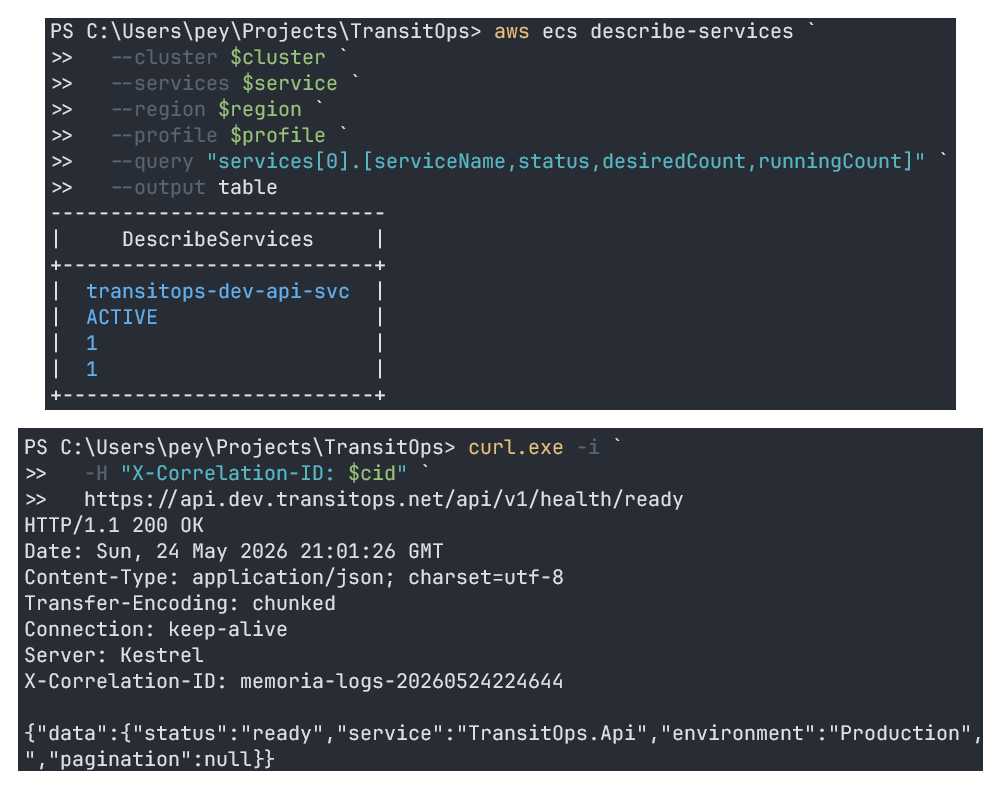
\includegraphics[width=0.92\textwidth]{imaxes/cloud-smoke-evidence}
\caption{Evidencia de servicio cloud operativo: ECS estable y readiness HTTPS con respuesta 200.}
\label{fig:cloud-smoke-evidence}
\end{figure}

\section{Evidencia de cierre de coste}
\label{sec:evidencia-cierre-coste}

Tras la validación de Sprint 6 se ejecutó \texttt{terraform destroy}. El primer intento eliminó la mayoría de recursos y falló al borrar ECR porque el repositorio contenía imágenes. Se vació el repositorio con \texttt{aws ecr batch-delete-image} y se repitió el destroy, que finalizó correctamente.

Tras Sprint 7 se repitió el cierre con la mejora \texttt{ecr\_force\_delete = true}. El destroy final eliminó \texttt{72} recursos y \texttt{terraform state list} no devolvió ningún recurso. Después se verificó que:

\begin{itemize}
  \item \texttt{terraform state list} no devolvía recursos.
  \item No quedaban ALB, RDS, ECS ni ECR asociados a \path{transitops-dev}.
  \item El NAT Gateway aparecía en estado \texttt{deleted}.
  \item No quedaban certificados ACM ni registros Route 53 de \endpoint{api.dev.transitops.net}.
  \item No quedaban log groups, dashboard, alarmas, snapshots temporales ni secretos del entorno \texttt{dev}.
\end{itemize}

Permanecen fuera de este destroy el dominio registrado \path{transitops.net}, su hosted zone pública y el backend remoto de Terraform, ya que son recursos de base necesarios para recreaciones posteriores y no forman parte del stack efímero de aplicación.

\section{Validación Sprint 8}
\label{sec:validacion-sprint8}

Sprint 8 completa la validación operativa con dos scripts de auditoría y un conjunto de runbooks. La recreación real partió de un state vacío, creó \texttt{72} recursos con ECS a cero tareas, publicó la imagen \tech{sprint8-good-fdf98b9}, cargó secretos runtime y ejecutó la tarea ECS de migración con exit code \texttt{0}. Después se escaló el servicio a \texttt{desired = 1} y \texttt{running = 1}, usando la task definition \tech{transitops-dev-api:9}.

La validación funcional confirmó readiness HTTPS \texttt{200} con correlation id \tech{sprint8-health}, bootstrap de administrador \texttt{201} con \tech{sprint8-bootstrap} y login \texttt{200} con \tech{sprint8-login}. CloudWatch contenía logs JSON filtrables por ese identificador, el dashboard \tech{transitops-dev-api}, 9 alarmas, topic SNS y suscripción de email en estado \texttt{PendingConfirmation}. Antes de destruir, \texttt{terraform plan -detailed-exitcode} no mostró cambios pendientes.

La auditoría de seguridad verificó que RDS no era público, ECS no tenía IP pública, los grupos de seguridad mantenían el flujo Internet--ALB--ECS--RDS, los secretos runtime existían en Secrets Manager y el rol de aplicación no contenía políticas inline. El rol OIDC de despliegue conserva permisos amplios para ejecutar Terraform en \texttt{dev}; se documenta como riesgo aceptado porque la trust policy queda limitada al repositorio y rama configurados.

También se revisa el coste del entorno. Los recursos que generan coste mientras \texttt{dev} está activo son principalmente NAT Gateway, ALB, ECS Fargate, RDS, CloudWatch, Secrets Manager y ECR. El cierre obligatorio del sprint volvió a ejecutar \texttt{terraform destroy}, eliminó \texttt{72} recursos y después comprobó la ausencia de ALB, ECS, RDS, ECR, certificado ACM, registros \path{api.dev}, logs, dashboard, alarmas, secretos y snapshots temporales. Los secretos runtime se borraron de forma forzada tras quedar inicialmente programados para eliminación por Secrets Manager. La Figura~\ref{fig:sprint8-cost-review} muestra la revisión de costes por servicio durante la recreación temporal del entorno, confirmando qué recursos generan gasto y en qué proporción. La Figura~\ref{fig:sprint8-destroy-audit} muestra el resultado de la auditoría post-destroy que verifica la ausencia de recursos efímeros asociados al stack \path{transitops-dev}.

\begin{figure}[htbp]
\centering
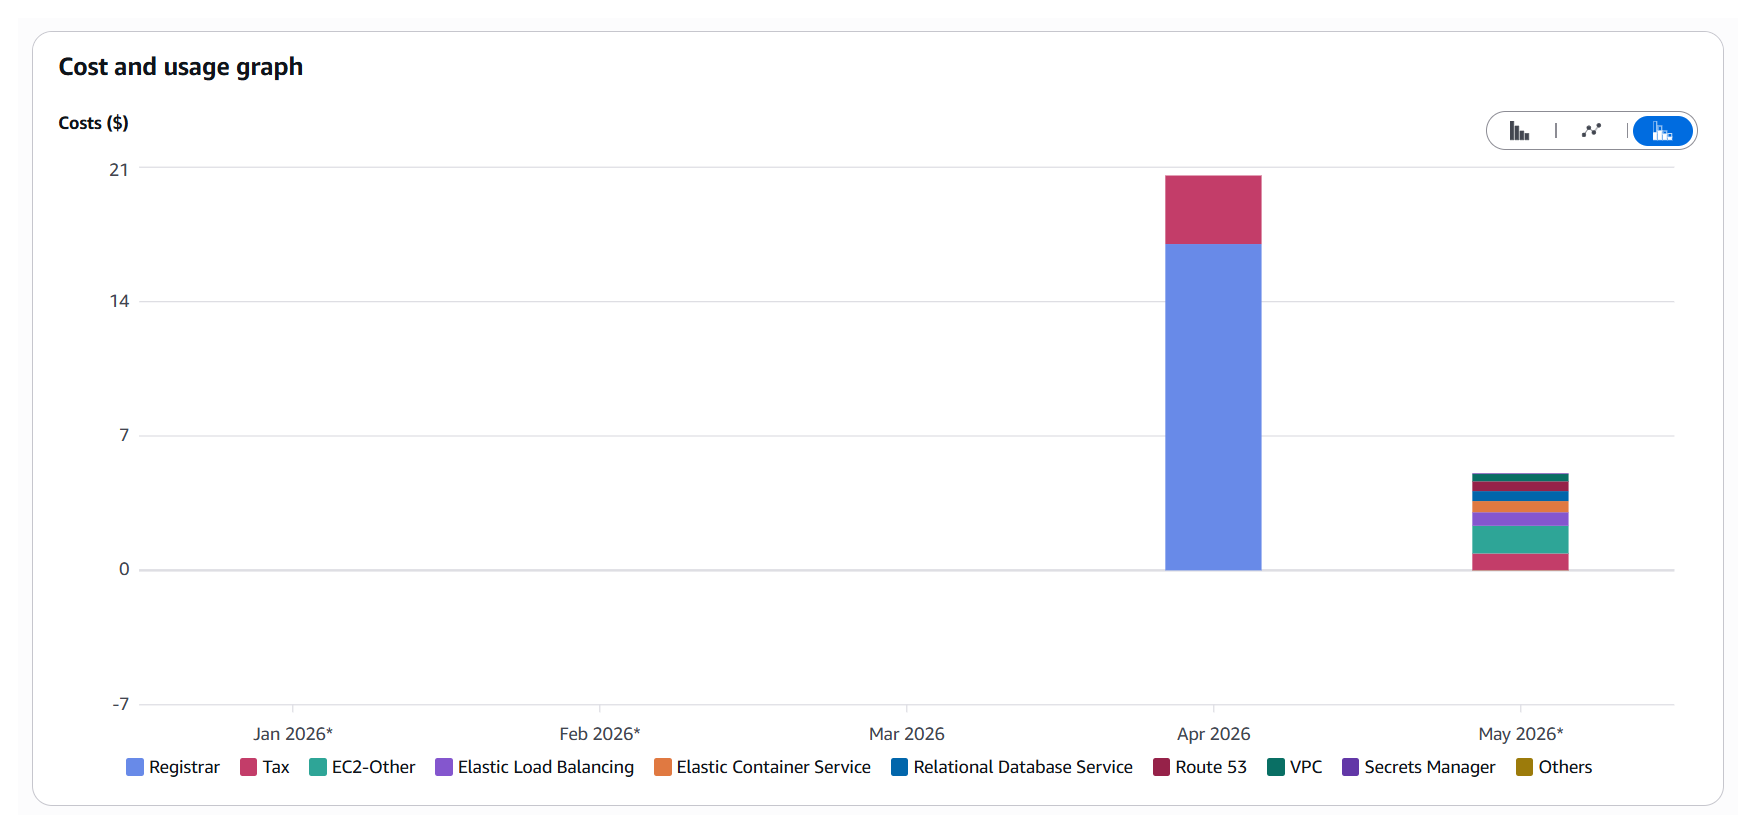
\includegraphics[width=0.92\textwidth]{imaxes/cost-review}
\caption{Evidencia de revisión de coste Sprint 8.}
\label{fig:sprint8-cost-review}
\end{figure}

\begin{figure}[htbp]
\centering
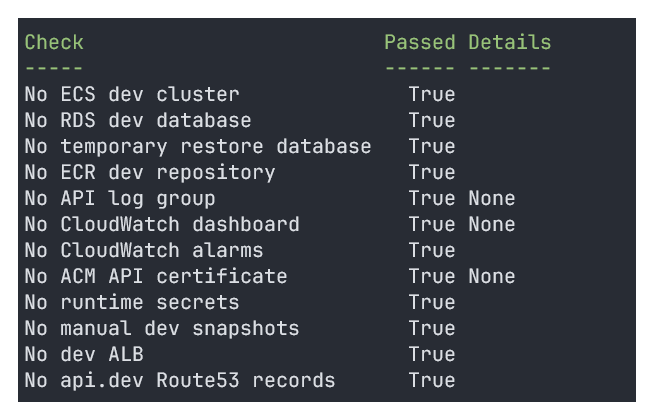
\includegraphics[width=0.92\textwidth]{imaxes/destroy-audit}
\caption{Evidencia de auditoría post-destroy Sprint 8.}
\label{fig:sprint8-destroy-audit}
\end{figure}

\section{Análisis de limitaciones}
\label{sec:analisis-limitaciones}

Las principales limitaciones son:

\begin{itemize}
  \item No existe interfaz gráfica; el sistema se consume mediante API, Postman o clientes equivalentes.
  \item El entorno desplegado es \texttt{dev}, no una arquitectura productiva multi-entorno completa.
  \item No se han implementado políticas de autoscaling ni pruebas de carga.
  \item La observabilidad cubre logs JSON, correlación, dashboard y alarmas básicas, pero no incluye trazas distribuidas ni APM completo.
  \item La evidencia visual incorporada cubre despliegue, DNS/HTTPS, observabilidad, rollback, restore, coste y auditoría post-destroy.
  \item Algunas políticas IAM son prácticas para el sprint actual y pueden afinarse más en fases posteriores.
\end{itemize}

\section{Cierre Sprint 9}
\label{sec:cierre-sprint9}

El cierre final del proyecto organiza la evidencia y la trazabilidad de forma explícita. Se añade una matriz que relaciona requisitos funcionales y no funcionales con implementación, pruebas y evidencia documental. También se prepara un índice final de evidencias y un guion de verificación para poder repetir localmente las comprobaciones principales o, si se necesitan capturas frescas, recrear brevemente el entorno \texttt{dev}, validar HTTPS, login, observabilidad y destruirlo de nuevo.

Los documentos principales de cierre son:

\begin{itemize}
  \item \path{docs/RequirementsTraceability.md}: matriz FR/NFR frente a implementación, verificación y evidencia.
  \item \path{docs/FinalEvidence.md}: índice de evidencias reales y capturas incorporadas.
  \item \path{docs/FinalVerification.md}: checklist local, ruta opcional de recreación AWS y guion de defensa técnica.
\end{itemize}

Este cierre evita que la defensa dependa de memoria de sesión o de una explicación oral improvisada. La relación entre alcance, implementación, operación y evidencias queda registrada en el repositorio.
